\chapter{First steps outside the Local Group of Galaxies:Red Supergiants in NGC\,55}
\label{ch:ngc55}

% \textbf{Completeness:} \textbf{30\%} \\
% The observations for this section are complete and the data reduction is
% currently being optimised.

% \textbf{Description:} \\
% This chapter will outline KMOS observations of 20 RSGs in NGC\,55.
% I will descibe the work I have done in preperation for these observations.

% I will discuss the optimisations which have been made for this data set and
% describe the challenges of obtaining the best possible data from a set of
% challenging observations.

% I will comment on the spatial distribution of the chemical abundances in this
% galaxy and discuss a potential metallicity gradient previously suggested in
% the literature.

\section{Opening Remarks} % (fold)
\label{sec:ngc55open}

Owen has kindly helped reconstruct and combine the data sets

% section opening_remarks (end)

\section{Introduction} % (fold)
\label{sec:ngc55intro}

NGC\,55 is a galaxy located outside of the Local Group of Galaxies within the Sculptor Group at a distance of 1.94\,$\pm$\,0.03\,Mpc~\citep{2006AJ....132.2556P,2008ApJ...672..266G} which, before the emergence of the Araucaria Project~\citep{2005Msngr.121...23G}, had been subject to considerable uncertainty~\citep[e.g.][]{1987ApJ...323...79P,2006A&A...455..891V}.

The Sculptor Group is considered to be the closest group of galaxies to our own and offers a fantastic laboratory with which to test theories of stellar and galactic evolution as using an 8-m class telescope, one can resolve individual stars within this group.
Association to the Sculptor group however, is a contentious issue.
Distance estimates vary to each galaxy, but typically when one references this group the main galaxies associated to this reference are: NGC\,55, NGC\,247, NGC\,253, NGC\,300 and NGC\,7793.
Where NGC\,253 is a large starbust galaxy which is the brightest and most dominant galaxy within this group.
In addition to these five large spiral galaxies, there are also numerous ($\sim$20) dwarf galaxies associated to this group.

By revising distances for nine of these dwarfs~\cite{2003A&A...404...93K} postulated that the Sculptor group was actually more like a filament of galaxies, which intersects the Milky Way group, where NGC\,55 and NGC\,300 and their surrounding satellite galaxies were potentially not associated with the main group of galaxies in this filament.
Regardless of the geometry and association to the Sculptor Group, NGC\,55 is the nearest large galaxy to the MW group in the direction of the Sculptor Group.

The morphology of NGC\,55 is asymmetric and complicated owing to the high inclination angle~\cite[up to 80\textdegree;][]{1986A&A...166...97H,2013MNRAS.434.3511W}.
\cite{1961ApJ...133..405D} classified this galaxy as an LMC-like spiral barred galaxy (SB(s)m) where the bar is seen along the line of sight~\cite{1961ApJ...133..405D}
prompting various claims that this galaxy is an edge on analogue of the LMC~\citep[e.g.][although not cited heavily -- two citations in 50 years -- the idea has propagated]{1964IAUS...20..276R}.
Figure~\ref{fig:ngc55-wide} shows NGC\,55 and its complicated morphology where one can see the edge-on disk along the major axis of the galaxy and the brighter central part of the galaxy represents the head of the bar.
In addition, to NGC\,55 being orientated nearly edge on, extending from the disk-bar system there exists many star formation features such as giant H\,\2 regions as well as supergiant filaments and shells which are thought to allow ionising radiation to be transported to the halo where star-formation is currently occurring~\citep{1996AJ....112.2567F}.

\begin{figure}
 \centering
 \includegraphics[width=0.65\textwidth]{ngc55/eso0914a}
 \caption[Image of NGC\,55]{Image of NGC\,55 where the edge on disk of the galaxy makes up the major axis and the bright central region represents the head of the bar containing intense star forming regions.
 Image from the Wide Field Imager on the 2.2-metre MPG/ESO telescope at ESO La Silla Observatory. Credit: ESO, press release.}
 \label{fig:ngc55-wide}
\end{figure}


The morphology of NGC\,55, as well as its known population of massive hot stars~\citep{2008A&A...485...41C,2012A&A...542A..79C}, points to a recent history of intense star formation.
This is supported by the infrared morphology of NGC\,55 which is dominated by young star forming features~\citep[][with a star formation rate of 0.22\,M$_{\odot}$yr$^{-1}$]{2004ApJS..154..248E} as well as indications from near-IR imaging~\citep{2005ApJ...622..279D}.

The metal content of NGC\,55 is expected to be LMC-like, which is supported by~\cite{2012A&A...542A..79C} who measured metallicities of 12 blue supergiants using optical spectroscopy and found a mean metallicity [Z]~=~$-$0.40\,$\pm$\,0.13\,dex.
In addition,~\cite{1983MNRAS.204..743W} measure abundances of seven H\,\2 regions across the disk of NGC\,55 using the strong-line method (as well as four measurements of the auroral ``direct'' line method) and found a similar LMC-like metallicity.

Even though the hot massive star population of NGC\,55 has been explored,
there currently exists no confirmed RSGs in NGC\,55, although ~\cite{2005ApJ...622..279D} note that the near-IR CMDs of fields within the disk of NGC\,55 reveal signatures of RSGs.
This study represents the first quantitative study of RSGs in NGC\,55 and, by measuring metallicities of this population, will provide a crucial test of the metallicity gradient within this galaxy.

In this chapter I describe the observations undertaken in Section~\ref{sec:ngc55obs} and highlight the target selection method and its uncertainties.
Section~\ref{sec:ngc55data_red} details the data reduction process and its complications owing to the poor S/N ratios of the observations.
I then present the main results of the chapter in Section~\ref{sec:ngc55results} where I first measure radial velocities for each epoch of the RGSs, confirming their membership to NGC\,55, and then go on to measure stellar parameters for each target using the $J$-band analysis technique described in detail in Chapter~\ref{ch:janal}.
Section~\ref{sec:ngc55disc} presents a discussion of the results and the main conclusions are presented in Section~\ref{sec:ngc55conc}.

% section introduction (end)

\section{Observations} % (fold)
\label{sec:ngc55obs}

\subsection{Target Selection} % (fold)
\label{sub:target_selection}

% In order to select RSG candidates in NGC\,55 I compiled optical photometry from two sources: The Araucaria Project~\citep{2005Msngr.121...23G} and the ACS Nearby Galaxy Survey Treasury project~\citep[ANGST][]{2009ApJS..183...67D}.
% Figure~\ref{fig:ngc55-foot} displays the footprints of the two projects.

% \begin{itemize}
%   \item Describe the two projects and their limitations:
%   \item Araucaria: Wide field ground-based with the aim of measuring distances using Cephieds and BSGs
%   \item ANGST: deeper HST survey of nearby (<4\,Mpc) galaxies covering some of the disk in NGC\,55.
%   \item Selected based on cuts in the ANGST photometry and then applied to the ground based survey
% \end{itemize}


Targets were selected based on the optical photometry from the ACS Nearby Galaxy Survey Treasury~\citep[blue; ANGST][]{2009ApJS..183...67D} project.
The optical CMD which is used to select targets is displayed in Figure~\ref{fig:VI}, where the RSG candidates are within the black box and the observed targets are highlighted in red.
This method of target selection is preferred as a result of the limited extent of near-IR photometry in this area.
The ANGST project publicly available photometry for several fields within the disk of NGC\,55 that are displayed as small white squares in Figure~\ref{fig:ngc55-foot}, overlaid on a DSS image.
In addition to the ANGST HST photometry, ground-based optical photometry is obtained from the Araucaria Project which covers the full spatial extent of NGC\,55 (large white rectangles in Figure~\ref{fig:ngc55-foot}).

\begin{figure}
 \centering
 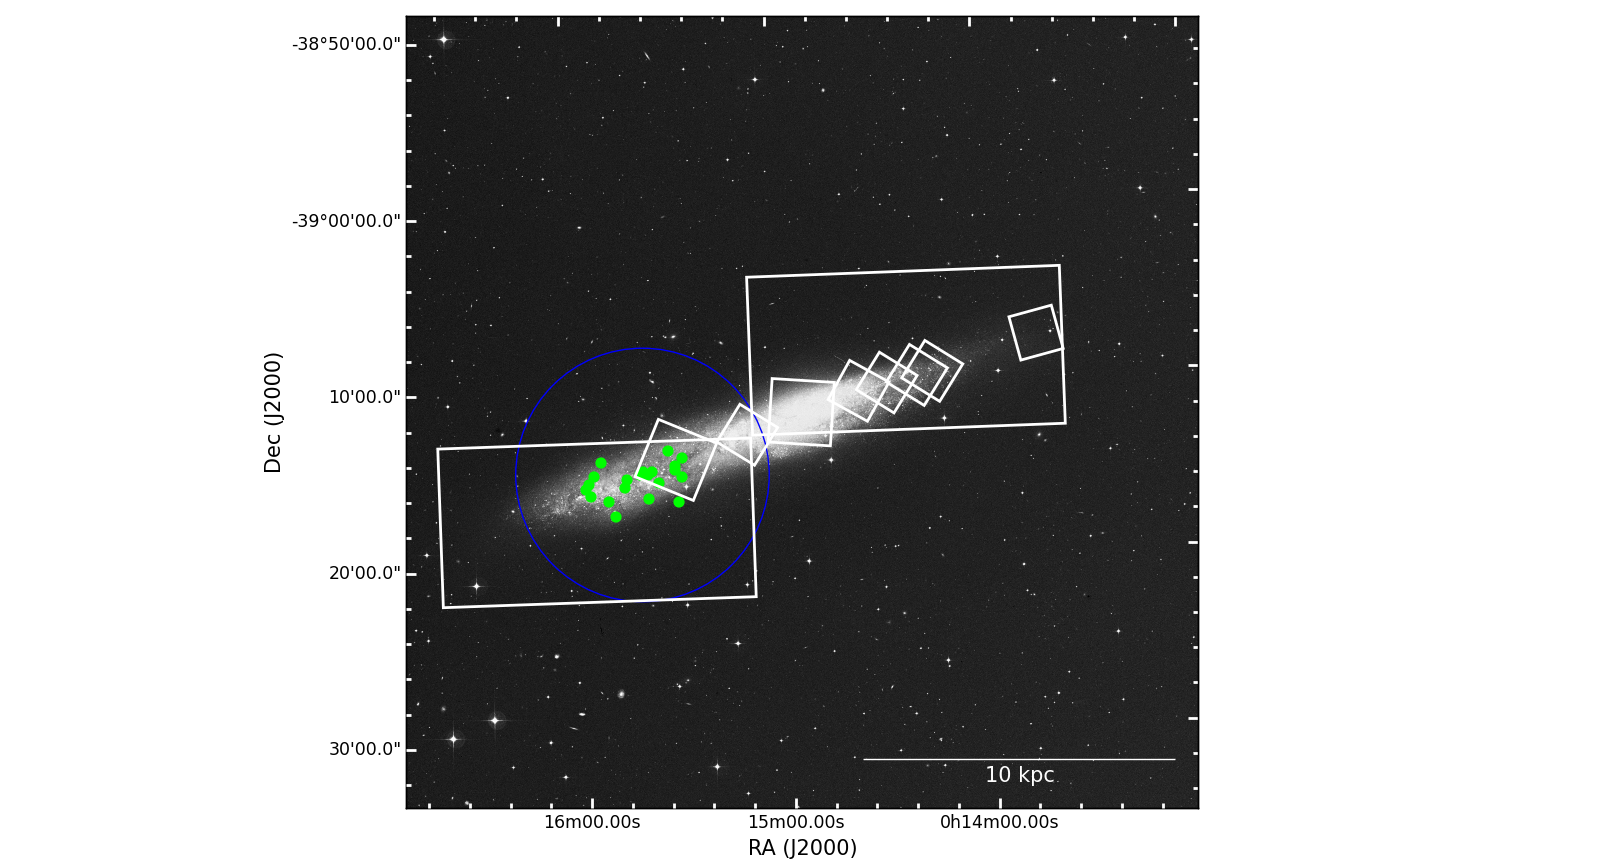
\includegraphics[width=\textwidth]{ngc55/ngc55_fields-v3}
 \caption[DSS image of NGC\,55 with KMOS and photometric footprints highlighted]{
          DSS image of NGC\,55 with KMOS targets overlaid in green and photometric footprints from the Araucaria Project
          \protect\citep{2005Msngr.121...23G} in white rectangles
          and the ANGST project
          \protect\citep{2009ApJS..183...67D} in the smaller white squares.
         }
 \label{fig:ngc55-foot}
\end{figure}

The selection criteria used in this study makes is based optical $F606-F814$ colours and $F814$ magnitudes.
Owing to their cool temperatures and extreme luminosities RSGs are known to exist in a ``plume'' at the tip of a structure of cool stars in the $F606-F814$, $F814$ CMD~\citep[e.g.][]{2015ApJ...805..182G}.
Figure~\ref{fig:VI} displays this CMD and the region of parameter space where RSG candidates reside is marked with a grey box.
This box has the limits $17 < F814 < 19$ and $1.2 < F606-F814 < 3.5$ following~\cite{2015ApJ...805..182G}, where the faint magnitude limit is chosen to select only targets which will have a S/N~=~100 in the original observing proposal.
As with selection criteria in the near-IR, the lower limit of this criteria is contaminated with a population of super-AGB stars which can have luminosities comparable to the faintest RSGs~\citep[e.g.][]{2000ApJ...542..804N}.
However, as stated in Chapter~\ref{ch:n6822} these stars are known to have lifetimes similar to the lowest mass RSGs and arguably still trace the young stellar population of this galaxy.

\begin{figure}
  \centering
  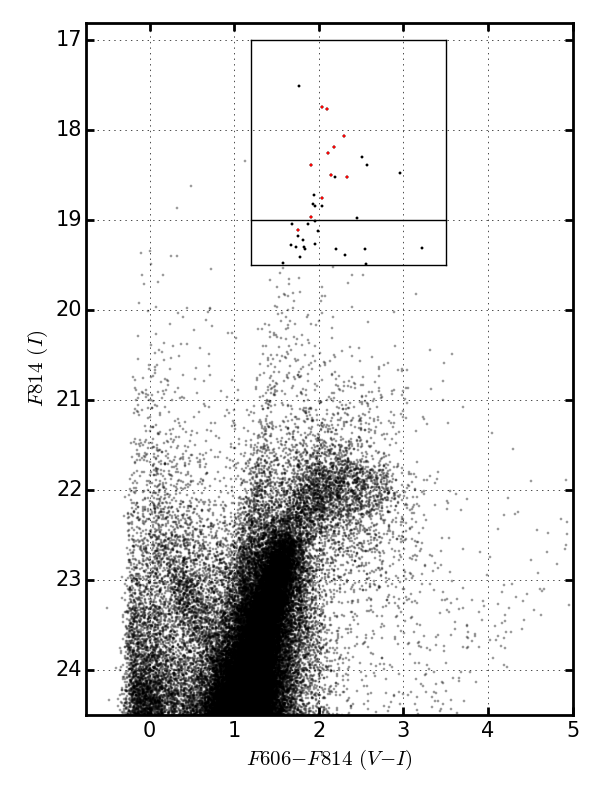
\includegraphics[width=0.45\textwidth]{ngc55/ngc55-v_i_angst}
 \caption[NGC\,55 $V-I$ colour--magnitude diagram]{
  NGC\,55 $V-I$ colour--magnitude diagram from the ACS Nearby Galaxy Survey Treasury~\citep[ANGST][]{2009ApJS..183...67D} project.
  The black box defines the selection criteria for candidate RSGs, which is defined as $17 < F814 < 19$ and $1.2 < F606-F814 < 3.5$.
  The lower-panel of the black box defines priority 2 RSG candidates.
          }
 \label{fig:VI}
\end{figure}


% \begin{figure}
%  \begin{center}$
%   \centering
%   \begin{array}{cc}
%   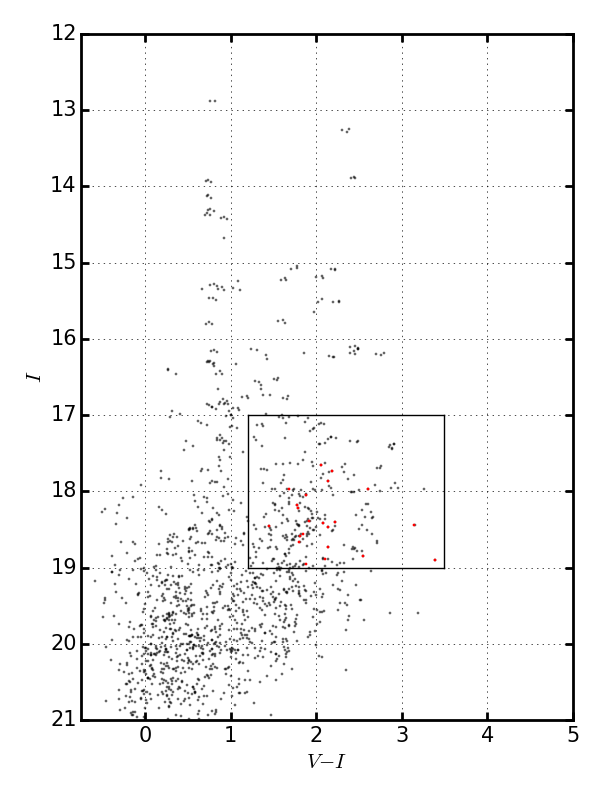
\includegraphics[width=0.45\textwidth]{ngc55/ngc55-v_i_ara} &
%   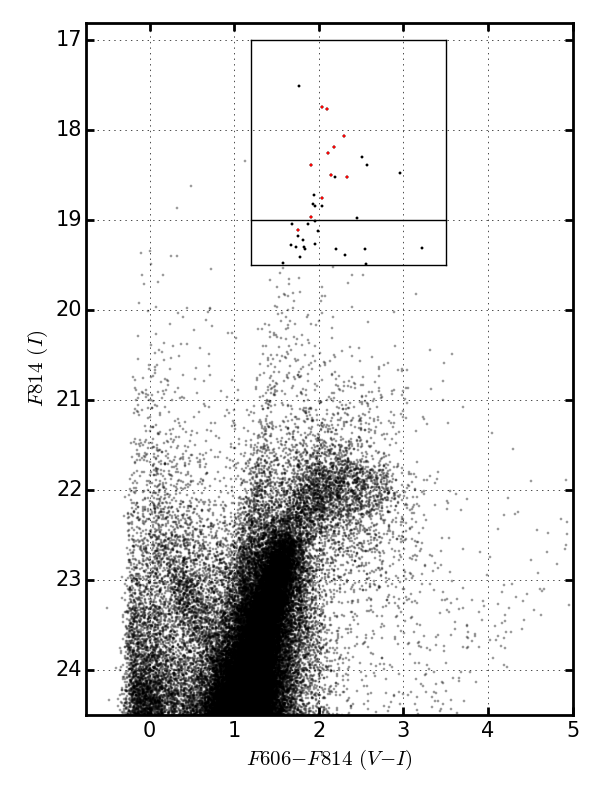
\includegraphics[width=0.45\textwidth]{ngc55/ngc55-v_i_angst} \\
%   \end{array}$
%  \end{center}
%  \caption[NGC\,55 ground- and space-based CMDs]{
%   NGC\,55 ground- and space-based $V-I$ against $I$ CMDs. Left hand panel shows data from the ground-based Araucaria Project~\cite{2005Msngr.121...23G}
%   over the entire FoV of the KMOS observations.
%   Right hand panel shows data from the ANGST project~\citep[blue; ANGST][]{2009ApJS..183...67D} where photometry from this project covers only a portion of the KMOS FoV.
%   The black boxes in each panel define candidate RSGs, which are defined as $17 < F814 < 19$ and $1.2 < F606-F814 < 3.5$ in the right hand panel and consequently applied to a larger FoV in the left hand panel assuming a one-to-one relationship between the ground- and space-based filters.
%           }
%  \label{fig:VI}
% \end{figure}


Table~\ref{tb:n55obs-params} shows ground- and space-based optical photometry of the KMOS targets along with their radial velocities which confirm many of these targets as NGC\,55 RSGs (see section~\ref{sub:rvs}).



\begin{sidewaystable}
\caption[Summary of VLT-KMOS targets in NGC\,55]{Summary of VLT-KMOS targets in NGC\,55.\label{tb:n55obs-params}}
\scriptsize
\begin{threeparttable}
\centering
\begin{tabular}{lrcccccccccccl}
 \hline
 \hline
ID & S/N & $\alpha$ (J2000) & $\delta$ (J2000) & $V$\tnote{a} & $I$\tnote{a} & $F606$\tnote{b} & $F814$\tnote{b} & \multicolumn{4}{c}{$rv$ (\kms)} & $\langle rv\rangle$ (\kms) & Notes \\
\cline{9-12}
& &  & & & & & & 14-09-2013 & 16-10-2013 & 14-09-2014 & 15-09-2014\\

 \hline
NGC55-RSG19 & xx & 00:15:29.190 & $-$39:14:08.20& 19.914 & 17.731 &19.85 & 17.76 &   205\,$\pm$\,4  &  178\,$\pm$\,7   &    222\,$\pm$\,10 &   191\,$\pm$\,7               & 199\,$\pm$\,14 & Notes\\
NGC55-RSG20 & xx & 00:15:29.520 & $-$39:15:13.00& 20.832 & 18.952 &20.86 & 19.11 &   194\,$\pm$\,14 &  220\,$\pm$\,5   & -- & --                                           & 217\,$\pm$\,10 & Notes\\
NGC55-RSG22 & xx & 00:15:30.520 & $-$39:16:36.70& 20.406 & 18.589 & --   & --    &    95\,$\pm$\,14 &$-$41\,$\pm$\,26  & -- & --                                           & --             & Notes\\
NGC55-RSG24 & xx & 00:15:31.460 & $-$39:14:46.30& 20.612 & 18.475 &20.29 & 18.38 &   186\,$\pm$\,6  &  194\,$\pm$\,7   &    146\,$\pm$\,38 &   237\,$\pm$\,16              & 192\,$\pm$\,16 & Notes\\
NGC55-RSG25 & xx & 00:15:31.490 & $-$39:14:32.40& 20.316 & 18.394 &20.63 & 18.49 &   204\,$\pm$\,12 &  217\,$\pm$\,16  & $-$376\,$\pm$\,41\tnote{c} & 151\,$\pm$\,23       & 200\,$\pm$\,26 & Notes\\
NGC55-RSG26 & xx & 00:15:33.160 & $-$39:13:42.00& 20.572 & 17.964 &20.35 & 18.06 &   174\,$\pm$\,9  &  173\,$\pm$\,8   & -- & --                                           & 173\,$\pm$\,1  & Notes\\
NGC55-RSG28 & xx & 00:15:36.160 & $-$39:15:29.40& 21.001 & 18.892 &20.87 & 18.97 &   233\,$\pm$\,17 &  161\,$\pm$\,20  & -- & --                                           & 203\,$\pm$\,41 & Notes\\
NGC55-RSG30 & xx & 00:15:38.030 & $-$39:14:50.20& 20.867 & 18.730 &20.79 & 18.75 &   212\,$\pm$\,10 &  215\,$\pm$\,10  & $-$424\,$\pm$\,21\tnote{c} & 212\,$\pm$\,22       & 213\,$\pm$\,2  & Notes\\
NGC55-RSG35 & xx & 00:15:39.260 & $-$39:15:01.70& 20.007 & 17.872 &19.78 & 17.73 &   202\,$\pm$\,3  &  206\,$\pm$\,4   &    223\,$\pm$\,13 &   200\,$\pm$\,11              & 204\,$\pm$\,5  & Notes\\
NGC55-RSG36 & xx & 00:15:39.520 & $-$39:16:23.10& 19.915 & 18.462 & --   & --    &$-$188\,$\pm$\,31 &$-$284\,$\pm$\,16 & $-$588\,$\pm$\,35 &   346\,$\pm$\,12              & --             & Notes\\
NGC55-RSG39 & xx & 00:15:40.260 & $-$39:15:01.00& 19.654 & 17.970 &20.36 & 18.19 &   206\,$\pm$\,11 &  192\,$\pm$\,5&$-$1\,$\pm$\,30\tnote{c}& 126\,$\pm$\,30              & 193\,$\pm$\,14 & Notes\\
NGC55-RSG43 & xx & 00:15:40.700 & $-$39:14:50.20& 19.957 & 18.183 &20.36 & 18.25 &$-$220\,$\pm$\,20\tnote{c}&196\,$\pm$\,5& 173\,$\pm$\,17 &    31\,$\pm$\,38\tnote{c}     & 194\,$\pm$\,9  & Notes\\
NGC55-RSG46 & xx & 00:15:41.640 & $-$39:14:58.80& 21.591 & 18.441 &20.85 & 18.52 &   228\,$\pm$\,5  &  195\,$\pm$\,6   &  $-$128\,$\pm$\,18\tnote{c} &   210\,$\pm$\,8     & 214\,$\pm$\,18 & Notes\\
NGC55-RSG57 & xx & 00:15:45.590 & $-$39:15:16.40& 20.010 & 18.220 & --   & --    &   217\,$\pm$\,10 &  197\,$\pm$\,6   &     207\,$\pm$\,13 &   177\,$\pm$\,6              & 193\,$\pm$\,16 & Notes\\
NGC55-RSG58 & xx & 00:15:46.270 & $-$39:15:43.20& 20.619 & 18.400 & --   & --    &   236\,$\pm$\,8  &  216\,$\pm$\,3   &     214\,$\pm$\,21 &   210\,$\pm$\,13             & 218\,$\pm$\,8  & Notes\\
NGC55-RSG60 & xx & 00:15:49.180 & $-$39:17:19.80& 21.393 & 18.847 & --   & --    & $-$73\,$\pm$\,39 &   26\,$\pm$\,26  &  $-$533\,$\pm$\,39 &    94\,$\pm$\,37             & --             & Notes\\
NGC55-RSG65 & xx & 00:15:51.250 & $-$39:16:26.40& 19.706 & 17.653 & --   & --    &   224\,$\pm$\,5  &  215\,$\pm$\,4   &     217\,$\pm$\,6  &   215\,$\pm$\,6              & 218\,$\pm$\,4  & Notes\\
NGC55-RSG67 & xx & 00:15:53.110 & $-$39:14:13.60& 19.925 & 18.047 & --   & --    &25\,$\pm$\,24\tnote{c} & 6\,$\pm$\,31\tnote{c}&37\,$\pm$\,14\tnote{c} &175\,$\pm$\,18    & 175\,$\pm$\,18 & Notes\\
NGC55-RSG69 & xx & 00:15:55.280 & $-$39:15:00.10& 20.470 & 18.666 & --   & --    &   231\,$\pm$\,5  &  195\,$\pm$\,9   &130\,$\pm$\,14\tnote{c}&220\,$\pm$\,23             & 222\,$\pm$\,18 & Notes\\
NGC55-RSG70 & xx & 00:15:56.310 & $-$39:16:08.60& 22.300 & 18.907 & --   & --    &   155\,$\pm$\,12 &  187\,$\pm$\,9   &     202\,$\pm$\,20 &   205\,$\pm$\,24             & 180\,$\pm$\,20 & Notes\\
NGC55-RSG71 & xx & 00:15:56.900 & $-$39:15:27.50& 20.401 & 18.559 & --   & --    &   197\,$\pm$\,11 &  214\,$\pm$\,11  &320\,$\pm$\,16\tnote{c}&$-$476\,$\pm$\,42\tnote{c} & 206\,$\pm$\,12 & Notes\\
NGC55-RSG73 & xx & 00:15:57.710 & $-$39:15:41.50& 20.489 & 18.411 & --   & --    &   161\,$\pm$\,7  &  178\,$\pm$\,6   &     136\,$\pm$\,35 &   176\,$\pm$\,19             & 171\,$\pm$\,11 & Notes\\

\hline
\end{tabular}
\begin{tablenotes}
  \item [a] Ground based data from the Araucaria Project
  \protect\cite{2006AJ....132.2556P}, with typical photometric uncertainty 0.075 and 0.016 in $V$ and $I$ bands respectively.
  \item [b] HST ANGST photometry from
  \protect\cite{2009ApJS..183...67D}, with typical errors 0.12, 0.13 in $F606$ and $F814$ bands respectively.
  \item [c] Value excluded from average for target.
\end{tablenotes}
\end{threeparttable}
\end{sidewaystable}

% subsection target_selection (end)
\section{Observations and Data Reduction} % (fold)
\label{sec:ngc55:obs_data}

These observations are part of the the KMOS guaranteed time observations (GTO) (ESO ID: 092.B-0088(A)) that was proposed to measure spatial variations in metallicities NGC\,55 and NGC\,300 both at d~=~1.9\.Mpc.
This included three pointings in NGC\,55 containing $\sim$60 RSG candidates.
However, during the observations in October 2013, as a result of poor conditions, only half the requested time on one field in NGC\,55 was observed.
In order to supplement this partially completed OB, the proposal was re-submitted as a back-up OB for subsequent GTO.

As back-up observations, this OB was observed on two nights in August 2014.
Therefore, this OB was observed on four different nights: 14-10-2013, 16-10-2013, 14-09-2014 and 15-10-2014 as detailed by Table~\ref{tb:55obs}.
The observations on each night consisted of science exposures (S) with sky offset exposures (S) interveaved in an O, S, O observing pattern, where each exposure is 600\,s.

\begin{table}
\caption[NGC\,55 observing log]{NGC\,55 observing log.\label{tb:55obs}}
\scriptsize
\begin{center}
\begin{tabular}{ccccc}
\hline
\hline
Date & Seeing Conditions ($arcsec$) & Airmass & Number of Exposures & Notes\\
  \hline
14-10-2013 & 0\farcs8--1\farcs2 & 1.0--1.8 & 6~$\times$~600s & Observed by author\\
16-10-2013 & 0\farcs8--1\farcs2 & 1.0--1.3 & 14~$\times$~600s & Observed by author\\
14-09-2014 & 0\farcs4--2\farcs2 & 1.0--1.9 & 24~$\times$~600s & Back-up observations\\
15-09-2014 & 1\farcs1--1\farcs6 & 1.1--1.5 & 12~$\times$~600s & Back-up observations\\
\hline
\end{tabular}
\end{center}
\end{table}

In addition , on each night a standard set of KMOS calibration files was obtained as well as standard star observations on each night.
In October 2013 HIP\,3820~\citep[B8\,V;][]{1978mcts.book.....H} was observed using the 24-arm telluric template (KMOS\_spec\_acq\_stdstarscipatt).
However, on 14-10-2013, this OB was interrupted and several of the IFUs (particularly on detector two) were not observed with the 24-arm recipe: this OB was not repeated.

In August 2014 the 3-arm telluric tempate (KMOS\_spec\_cal\_stdstar) was observsed as opposed to the full 24-arm template. However, on both of these nights both HIP\,3820 and HIP\,18926~\citep[B3\,V;][]{1988mcts.book.....H} were observed as a standard star.

The quality of the observations taken on each night varies significantly.
The first set of observations (14-09-2013) were taken in excellent conditions where the seeing conditions were stable with good transparency.
As one would expect with back-up observations the conditions were not so idillic.
On both nights where this OB was observed as a back-up target, the conditions were varying significantly thoughout the night wtih patchy, sometimes significant, cloud coverage.

These differences in the quality of the data and in the actual execution of the observations must all be taken into account when the data is reduced.
In addition to differences in the observations arising from the conditions, there are also differences as a result of the time between the observations.
Table~\ref{tb:55res} shows the mean measured resolution and resolving power, at the appropriate rotator angles, for each night where the NGC\,55 data were taken.
This table shows that the resolution can vary significant between each night, particularly on detector three where the mean resolving power changes by a factor of 1/5.
Therefore, this must be taking into consideration when combining exposures on different nights.
This is solved by using a simple Gaussian filter (as first described in Chapter~\ref{ch:janal}) to degrade the resolution of the spectra to that of the lowest resolution spectrum within the data set.
For example, all spectra for a star in IFU 1 would be degraded to a resolution of 3302 before being combined into a master spectrum for the four nights.

\begin{table*}
\caption[Measured velocity resolution for each night]
{Measured velocity resolution and resolving power across each detector.\label{tb:55res}}
\scriptsize
\begin{center}
\begin{tabular}{ccrcccc}
\hline
\hline
Date & Det. & IFUs & \multicolumn{2}{c}{Ne\,\lam1.17700\,$\mu$m}
            & \multicolumn{2}{c}{Ar\,\lam1.21430\,$\mu$m} \\
& & & FWHM (\kms) & $R$ & FWHM (\kms) & $R$ \\
  \hline
  \\
           & 1 & 1-8 &   95.48\,$\pm$\,2.42 & 3140\,$\pm$\,80 &
                         90.71\,$\pm$\,2.09 & 3305\,$\pm$\,76 \\
14-10-2013 & 2 & 9-16 &  88.67\,$\pm$\,1.67 & 3381\,$\pm$\,64 &
                         86.35\,$\pm$\,1.84 & 3472\,$\pm$\,74 \\
           & 3 & 17-24 & 82.89\,$\pm$\,1.81 & 3617\,$\pm$\,79 &
                         80.56\,$\pm$\,2.11 & 3721\,$\pm$\,97 \\
                         \\
  \hline
  \\
           & 1 & 1-8 &   95.48\,$\pm$\,2.46 & 3140\,$\pm$\,81 &
                         90.78\,$\pm$\,2.12 & 3302\,$\pm$\,77 \\
16-10-2013 & 2 & 9-16 &  88.91\,$\pm$\,1.66 & 3371\,$\pm$\,63 &
                         86.30\,$\pm$\,1.85 & 3473\,$\pm$\,74 \\
           & 3 & 17-24 & 82.96\,$\pm$\,2.14 & 3612\,$\pm$\,76 &
                         80.77\,$\pm$\,2.14 & 3712\,$\pm$\,98 \\
                         \\
\hline
\\
           & 1 & 1-8 &   84.18\,$\pm$\,1.93 & 3561\,$\pm$\,82 &
                         81.76\,$\pm$\,2.15 & 3667\,$\pm$\,96 \\
14-09-2015 & 2 & 9-16 &  87.00\,$\pm$\,1.69 & 3446\,$\pm$\,67 &
                         84.67\,$\pm$\,1.93 & 3541\,$\pm$\,81 \\
           & 3 & 17-24 & 97.14\,$\pm$\,1.88 & 3086\,$\pm$\,60 &
                         94.85\,$\pm$\,2.01 & 3161\,$\pm$\,67 \\
                         \\

\hline
\\
           & 1 & 1-8 &   82.55\,$\pm$\,1.96 & 3632\,$\pm$\,86 &
                         80.41\,$\pm$\,2.30 & 3728\,$\pm$\,106\\
15-09-2014 & 2 & 9-16 &  88.08\,$\pm$\,1.78 & 3404\,$\pm$\,69 &
                         86.03\,$\pm$\,1.96 & 3485\,$\pm$\,80\o\\
           & 3 & 17-24 & 98.04\,$\pm$\,1.91 & 3058\,$\pm$\,59 &
                         96.74\,$\pm$\,2.05 & 3099\,$\pm$\,66\o\\
                         \\
\hline
\end{tabular}
\end{center}
\end{table*}

\textbf{Data recuction isn't finalised but the basic steps are not going to change}

The observations were reduced using the recipes provided by the Software Package for Astronomical Reduction with KMOS
\citep[SPARK;][]{2013A&A...558A..56D}.
The standard KMOS/esorex routines were used to calibrate and reconstruct the science and standard-star data cubes as outlined by
\cite{2013A&A...558A..56D} including a correction which corrects for the readout coloumn bias as well as enhancing the bad pixel mask following Turner et al. (in prep.).
Using the reconstrucuted data cubes the pipeline was used to extract science and sky spectra in a consistent way for all exposures.

Sky subtraction was performed using the ESO {\sc skycorr} package~\citep{2014A&A...567A..25N}.
{\sc skycorr} is an instrument independent tool that applies a scaling to a sky spectrum given a pair of observed and sky spectra in order to more accurately match the sky lines in the observed spcectrum and hence, provide a more accurate sky subtraction.
This works by adapting the reference sky spectrum to correct for differences as a result of temporal and spatial airglow variability
This software is specifically designed for observations at Cerro Paranal and has been shown to be an effective tool for various different science goals~\citep[e.g.][]{2014A&A...567A..25N,2015ApJ...805..182G,2016MNRAS.455.2028F,2016MNRAS.457.1468L}.



\begin{itemize}
    \item Telluric correction ...
\end{itemize}


Telluric correction has been performed by combining and reconstructing the telluric standard exposures using the standard pipeline routines.
To improve the performance of the telluric correction I use the method described in detail in Chapter~\ref{ch:n6822}.

As mentioned above, were multiple standard star OBs for each night of observing.
The telluric spectrum used to correct each science spectrum is determined on a star-by-star basis depending upon a visual inspection of the results of the correction.

% The observations for this study were taken using four nights of KMOS guaranteed time observations (GTO) containing xx RSG candidates, the first of which was taken in October 2013 as part of the observations which led to the publication of~\cite{2015ApJ...805..182G}.
% These data consisted of six science exposures (S) of 600\,s with sky offset exposures (S) interleaved in an O, S, O observing pattern.
% Seeing conditions for these data were good at 0\farcs8--1\farcs2 throughout the course of the observing block (OB).

% The second data set which is made use of in this chapter comes from two nights in September 2014 where the OB used in 2013 was used as backup observations for a programme which required excellent seeing ($<$\,0\farcs6).
% The seeing limits on our observations are more relaxed ($<$\,1\farcs5) which gave us an opportunity to make use of some slightly poorer quality KMOS data.
% On the first night in September 2014 where this OB was observed, the seeing conditions varied widly ($>$\,1\farcs6) prompting one observer to comment that ``this is the worst recorded seeing at Paranal!''.
% However, there are 24 science exposures where the seeing conditions were better than 2\farcs2, which are (potentially) useful.
% The final night of observing consisted of 12 exposures with seeing conditions varying between 1\farcs1--1\farcs6.

% In addition to the science exposures obtained, on each night a standard set of KMOS calibration files were obtained as well as standard star observations on each night.
% The standard star observing block for each night is slightly different where in October 2013 HIP\,3820~\citep[B8\,V;][]{1978mcts.book.....H} was observed using the 24-arm telluric template (KMOS\_spec\_acq\_stdstarscipatt).
% However, in September 2014 only the three-arm telluric template was observed (KMOS\_spec\_cal\_stdstar), this time with HIP\,18926~\citep[B3\,V;][]{1988mcts.book.....H} and HIP\,3820 on both nights.

% section observations_and_data_reduction (end)
% section observations (end)

\section{Results} % (fold)
\label{sec:ngc55results}

\subsection{Radial Velocities} % (fold)
\label{sub:rvs}
Radial velocities are measured using the method described first in Chapter~\ref{ch:n2100} where radial velocities are measured using several strong spectral features within the 1.16-1.21\,$\mu$m region.
Each of these spectral features is independently used to measure a radial velocity where the value quoted is the average of these measurements and the uncertainties are defined by the standard deviation of the measurements.
This method is known to work well on KMOS stellar spectra~\cite{2015ApJ...798...23L,2015ApJ...803...14P,2016arXiv160202702P}.

Estimated radial velocities from each KMOS pointing is listed in Table~\ref{tb:n55obs-params} alongside the average radial velocity for each target, where any significantly discrepant measurement has been excluded as a result of residuals in the spectrum perturbing the fit (marked by note c in Table~\ref{tb:n55obs-params}).
This is a particular problem on the night of 14-09-2014 where 7/20 velocity measurements were excluded.
Uncertainties quoted on the average are the standard deviation of the measurements on each night.
% The average radial velocity of the sample is 199\,$\pm$\,16\,\kms.
Three targets (NGC55-RSG22, NGC55-RSG36 and NGC55-RSG60) have been excluded from this average based on their unreliable radial velocity estimates.
Given the significant variability in these measurements on each night, an assessment on membership to NGC\,55 is impossible given the current data.
Therefore, henceforth, these targets are excluded from the sample.

Comparing the estimated velocities to previous measurements we find good agreement with velocities measured for $\sim$200 BSGs in NGC\,55 in~\citep{2008A&A...485...41C} as well as with measurements of the velocity from the H\,\1 gas~\citep{1991AJ....101..447P}.
The estimated radial velocities as a function of galactocentric distance is shown in Figure~\ref{fig:RvsRV} where previous measurements are also shown for comparison.
The radius at which the surface brightness first reach 25\,mag/arcsec$^2$ in the $B$-band~\citep[R$_{25}$ e.g.][]{2015eaci.book.....S} is shown for scale~\citep[$R_{25}$~=~16.2\,$\pm$\,0.4\,arcmin][]{1991rc3..book.....D}
We find no evidence for a systematic offset between the measurements of~\cite{2008A&A...485...41C} and those measured in this study.

\begin{figure}
 \centering
 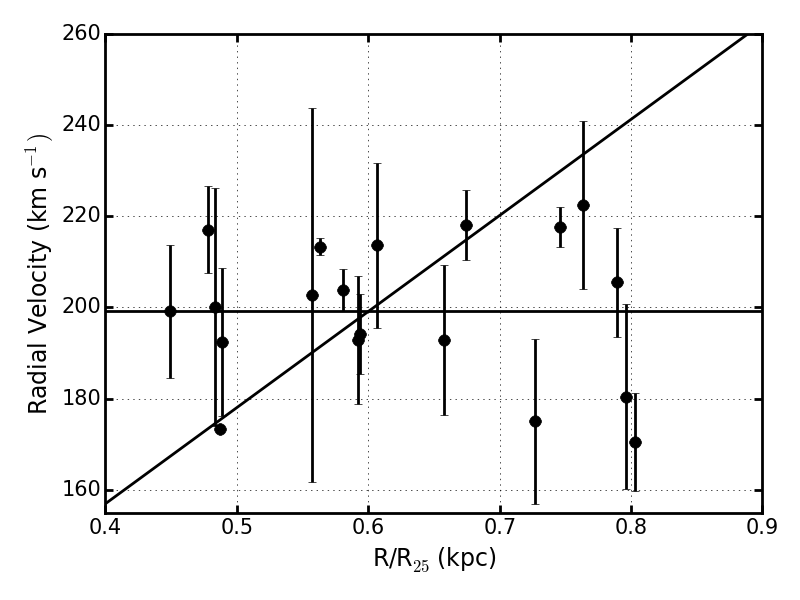
\includegraphics[width=0.65\textwidth]{ngc55/NGC55-RvsRV}
 \caption[Radial velocities for KMOS targets shown against projected radius]{
 Radial velocities for the KMOS RSGs (black points) shown against projected radius from the centre of NGC\,55 as defined by the Two Micron All Sky Survey~\citep[2MASS;][]{2006AJ....131.1163S} scaled by $R_{25}$~=~16.2\,$\pm$\,0.4\,arcmin~\citep{1991rc3..book.....D}.
Blue points show data for $\sim$200 BSGs in NGC\,55 from~\citep[][; shown with 50\% transparency to highlight densely populated areas]{2008A&A...485...41C} alongside the rotation curve of NGC\,55~\citep[black solid line;][]{1991AJ....101..447P}.}
 \label{fig:RvsRV}
\end{figure}

As the observed data is taken over four different epochs, the variability of each source can be assessed. No clear evidence for variability is found for any target within the observed sample.
To assess variability, the variability criteria of~\citep{2012A&A...546A..73H} is employed, i.e.

\begin{equation}
  \left|\frac{RV_i - \mu}{\sigma_i}\right| > 4.0,\label{eq:vary}
\end{equation}

\noindent where $RV_i$ is the radial velocity with an associated uncertainty  $\sigma_i$ measured on an individual night $i$ and $\mu$ is the average radial velocity for the target.
Using this criteria on all targets finds that no targets show evidence for variability.
This adds strength to the suggestion that observed RSGs are intrinsically single objects as a result of the length of time spent as a RSG in a binary is significantly decreased (see discussion in Chapter~\ref{ch:ngc2100}).


% subsection radial_velocities (end)
\subsection{Stellar Parameters} % (fold)
\label{sub:stellar_parameters}


\begin{itemize}
    \item Comparison to previous results
    \cite{2012A&A...542A..79C} find average [Z]~=~$-$0.4\,$\pm$\,0.13\,dex
    \item [Z] Vs. Radius from galaxy centre
    \item MCMC parameter estimation for the fit
    \item Extinction values need to be taken into account (especially if I'm estimating luminosities in the I band)
    \end{itemize}

Distance modulus~=~26.58\,$\pm$\,0.11~\citep{2011ApJ...738..150T}.
Distance modulus~=~26.434\,$\pm$\,0.037~\citep{2008ApJ...672..266G}

% subsection stellar_parameters (end)

% section results (end)

\section{Discussion} % (fold)
\label{sec:ngc55disc}

\begin{itemize}
    \item Orientation of NGC\,55
\end{itemize}
% section discussion (end)

\section{Conclusions} % (fold)
\label{sec:ngc55conc}

% section conclusions (end)

\bibliography{../journals,../books}